\documentclass[twocolumn]{article}

\title{Evaluation}
\usepackage{graphicx}
\usepackage[margin=0.75in]{geometry}
\usepackage{subcaption}
\usepackage{float}
\usepackage{blindtext}

\graphicspath{ {graphs/} }

\addtolength{\topmargin}{0.25in}
	\addtolength{\textheight}{-0.5in}

\begin{document}

\section[1]{Related Work}
	There are many existing tools that closely relate to Flair in their goals. We provide an overview of the most prevalent of those tools below:
	\subparagraph{Covert}
		Covert is a inter-application communication analysis tool which allows for the analyzing of inter-application vulnerabilities in android applications. It has been formulated to enable analysis of bundles of applications. It has two main processes. The first is model extraction where the tool extracts models from the APK files, and the second is that formal analyzer which processes those models and presents any vulnerabilities in an xml file\cite{Covert}.
	\subparagraph{DidFail}
		Didfail is a tool built off of another tool \textit{FlowDroid} \cite{Didfail}. Similar to Covert, it allows for the analysis of bundles of applications instead of just single applications, which was an improvement over \textit{FlowDroid}. Didfail consists of two phases of analysis. The first phase contains the tools Epicc, Dare, Soot, and FlowDroid. The second phase contains only TaintFlows \cite{Didfail}. Unlike the other tools, Didfail is unable to identify privilege escalation vulnerabilities within applications. 

	\subparagraph{DIALDroid}
		DIALDroid is an inter-application ICC security analysis tool with four key operations: ICC Entry / Exit Point Extraction, DataFlow Analysis, Data Aggregation, and ICC Leak Calculation\cite{DIALDroid}. DIALDroid extracts models from a given application and performs static analysis to find any ICC exit or entry leaks present. Then the information on any leaks is stored in a MySQL relational database to be retrieved via SQL queries. During the initial analysis stage DIALDroid changes the precision based on the length of the analysis. During the first five minutes of analysis DIALDroid uses a high precision algorithm to find ICC entry and exit leaks. After five minutes, DIALDroid switches to a low precision algorithm that has a higher chance of false negative. If the analysis runs for more than a given timeout, such as 15 minutes, DIALDroid abandons the analysis of that application altogether\cite{DIALDroid}.
	\subparagraph{SEALANT}
		SEALANT is an android security systems with the goal of both finding and preventing malicious android activity. It is composed of two tools: an analyzer and an interceptor. In this paper we focus only on the analyzer tool as it is closely related to our research. The analyzer works similarly to other ICC analysis tools. First, it extracts ICC paths from APK files. It then identifies vulnerable paths using formal analysis. Lastly, it enters the identified vulnerabilities into a list that will be used by the SEALANT interceptor tool.


\begin{center}
\section[2]{Empirical Evaluation}
\end{center}

\paragraph{•}
	We tested Flair's performance in relation to the following questions:\\
	\textbf{Question 1:} How does Flair compare to other inter-application communication analysis tools in respect to the amount of time it takes to analyze a bundle of applications?\\
	\textbf{Question 2:} How does Flair compare to other tools with respect to the number of applications it fails to analyze?\\
	\textbf{Question 3:} How accurately does Flair analyze privilege escalation vulnerabilities within applications when ran against a bundle of benchmark applications?\\
	\textbf{Question 4:} How does Flair's accuracy in analyzing privilege escalations compare to other inter-application communication analysis tools?\\

\subsection{Methods of Testing} \label{methods}
\paragraph{•}
	To test these questions we ran Flair four other inter-application analysis tools: Covert, Didfail, SEALANT, and DIALDroid. We used seven bundles of popular applications presented in table 1 android applications, each with fifty applications, to answer Question 1 and Questions 2. We then used two bundles of benchmark bundles also presented in table 1 to answer Question 3 and Question 4. 

\begin{table}[h]
\begin{center}
\begin{tabular}{ |c c| }
	\hline
	Bundle & Apks\\
	\hline
	Android Bundle 1 & 50\\
	Android Bundle 2 & 50\\
	Android Bundle 3 & 50\\
	Android Bundle 4 & 50\\
	Android Bundle 5 & 50\\
	Android Bundle 6 & 50\\
	Android Bundle 7 & 50\\
	DroidBench2.0 & 3\textbf{(Not Final)}\\
	ICC-Bench & 9\\
	\hline
\end{tabular}
\end{center}
\caption{Bundles used in analysis.}
\label{table:1}
\end{table}


\paragraph{•}
	Each of the bundles used to examine Question 1 and Question 2 were run incrementally. Each test started with only one application from the bundle and the tool was run against it. Then another application was added and the tool was run against the new bundle of two applications. This process was repeated until all the applications from the specified bundle were added. Therefore, each test bundle consisted of 50 consecutive runs of a tool, each consisting of one more application than the last. This was done to reflect how in a real world situation applications are added to a collection that is being checked for vulnerabilities. It is beneficial for us to see how each tool performs when new applications are added to a bundle. To more obtain more accurate results we ran each tool against each bundle three times and used the averages from those runs in our data.
\paragraph{•}
	We gathered data for Question 1 by recording the time it took each tool to analyze bundles of applications. We recorded the time each tool took for each successive run of a test. Hence, there was fifty recorded times for each test of a tool. The averages for each bundle were then entered into box plot graphs and evaluated.
\paragraph{•}
	To answer Question 2 we used error logs provided by each tool. The tools provided a single error log file for each application that they failed to analyze. We then calculated the failure rate of each tool by:\\
	\begin{center}
		\(\frac{failed}{num}=FR\)
	\end{center}
	Where \textit{failed} is the number of error logs given by the tool, \textit{num} is the total number of applications run in the test, here it is 1250, and \textit{FR} is the failure rate for that tool in that test. The failure rates were recorded for each test and then averaged for each tool across all bundles.
\paragraph{•}
	
	\textbf{Here will go text explaining Question 3 procedure.}
\paragraph{•}
	\textbf{Here will go text explaining Question 4 procedure.}

\subsection{Variables}
\paragraph{•}
	\textbf{Independent:} Our independent variables present in our test are as follows: (1) Tool used to analyze. (2) Specific bundle which the tool analyzed.\\
	\textbf{Dependent:} The dependent variables in our study are as follows: (1) Time it takes for tool to analyze a bundle. (2) Number of applications that a tool fails to analyze. (3) The accuracy of the analysis.
	
\subsection{Testing Environment}
	All testing for Question 1 and Question 2 was done on virtual machines running within Oracle VirtualBox. Each of these machines was running Ubuntu 16.04 and had 8 processing threads clocked at 2.28 Ghz. The memory varied due to the fact that each tool had differing memory requirements. For Covert, Didfail, and Flair the machine was given 3 GB of memory. SEALANT required more memory to run and was given 6 GB. DIALDroid, the most memory intensive, was given 14 GB. Since SEALANT and DIALDroid had much higher memory requirements than the other tools, we gave them the lower limit of the amount of memory that they needed to run. We did this so that each tool would have enough memory to run efficiently, but the higher memory requirement tools did not have a clear advantage. In addition, there was no swap space available for any of the tools.
	
\subsection{Threats to Validity}
\paragraph{•}
	\textbf{Inconsistent Runs:} Though we ran all tests in isolated virtual machines, there still could have been issues related to a run that is not consistent with the tools true performance. To minimize these affects we ran each tool against each bundle three times and took the averages.
\paragraph{•}
	\textbf{Internal issues:} Issues related to the structure and design of the tools themselves. We are not aware of any issues of this kind.
\paragraph{•}
	\textbf{Measurement Issues:} Issues related to the methods we used to record and analyze our data. We did not notice any issued related to this.
	
\clearpage
\newpage

\subsection{Results}

%Figure that represents the box plot graphs of all the Tools
\begin{figure}[ht]
\onecolumn
\centering
	\begin{subfigure}{0.5\textwidth}
		\centering
		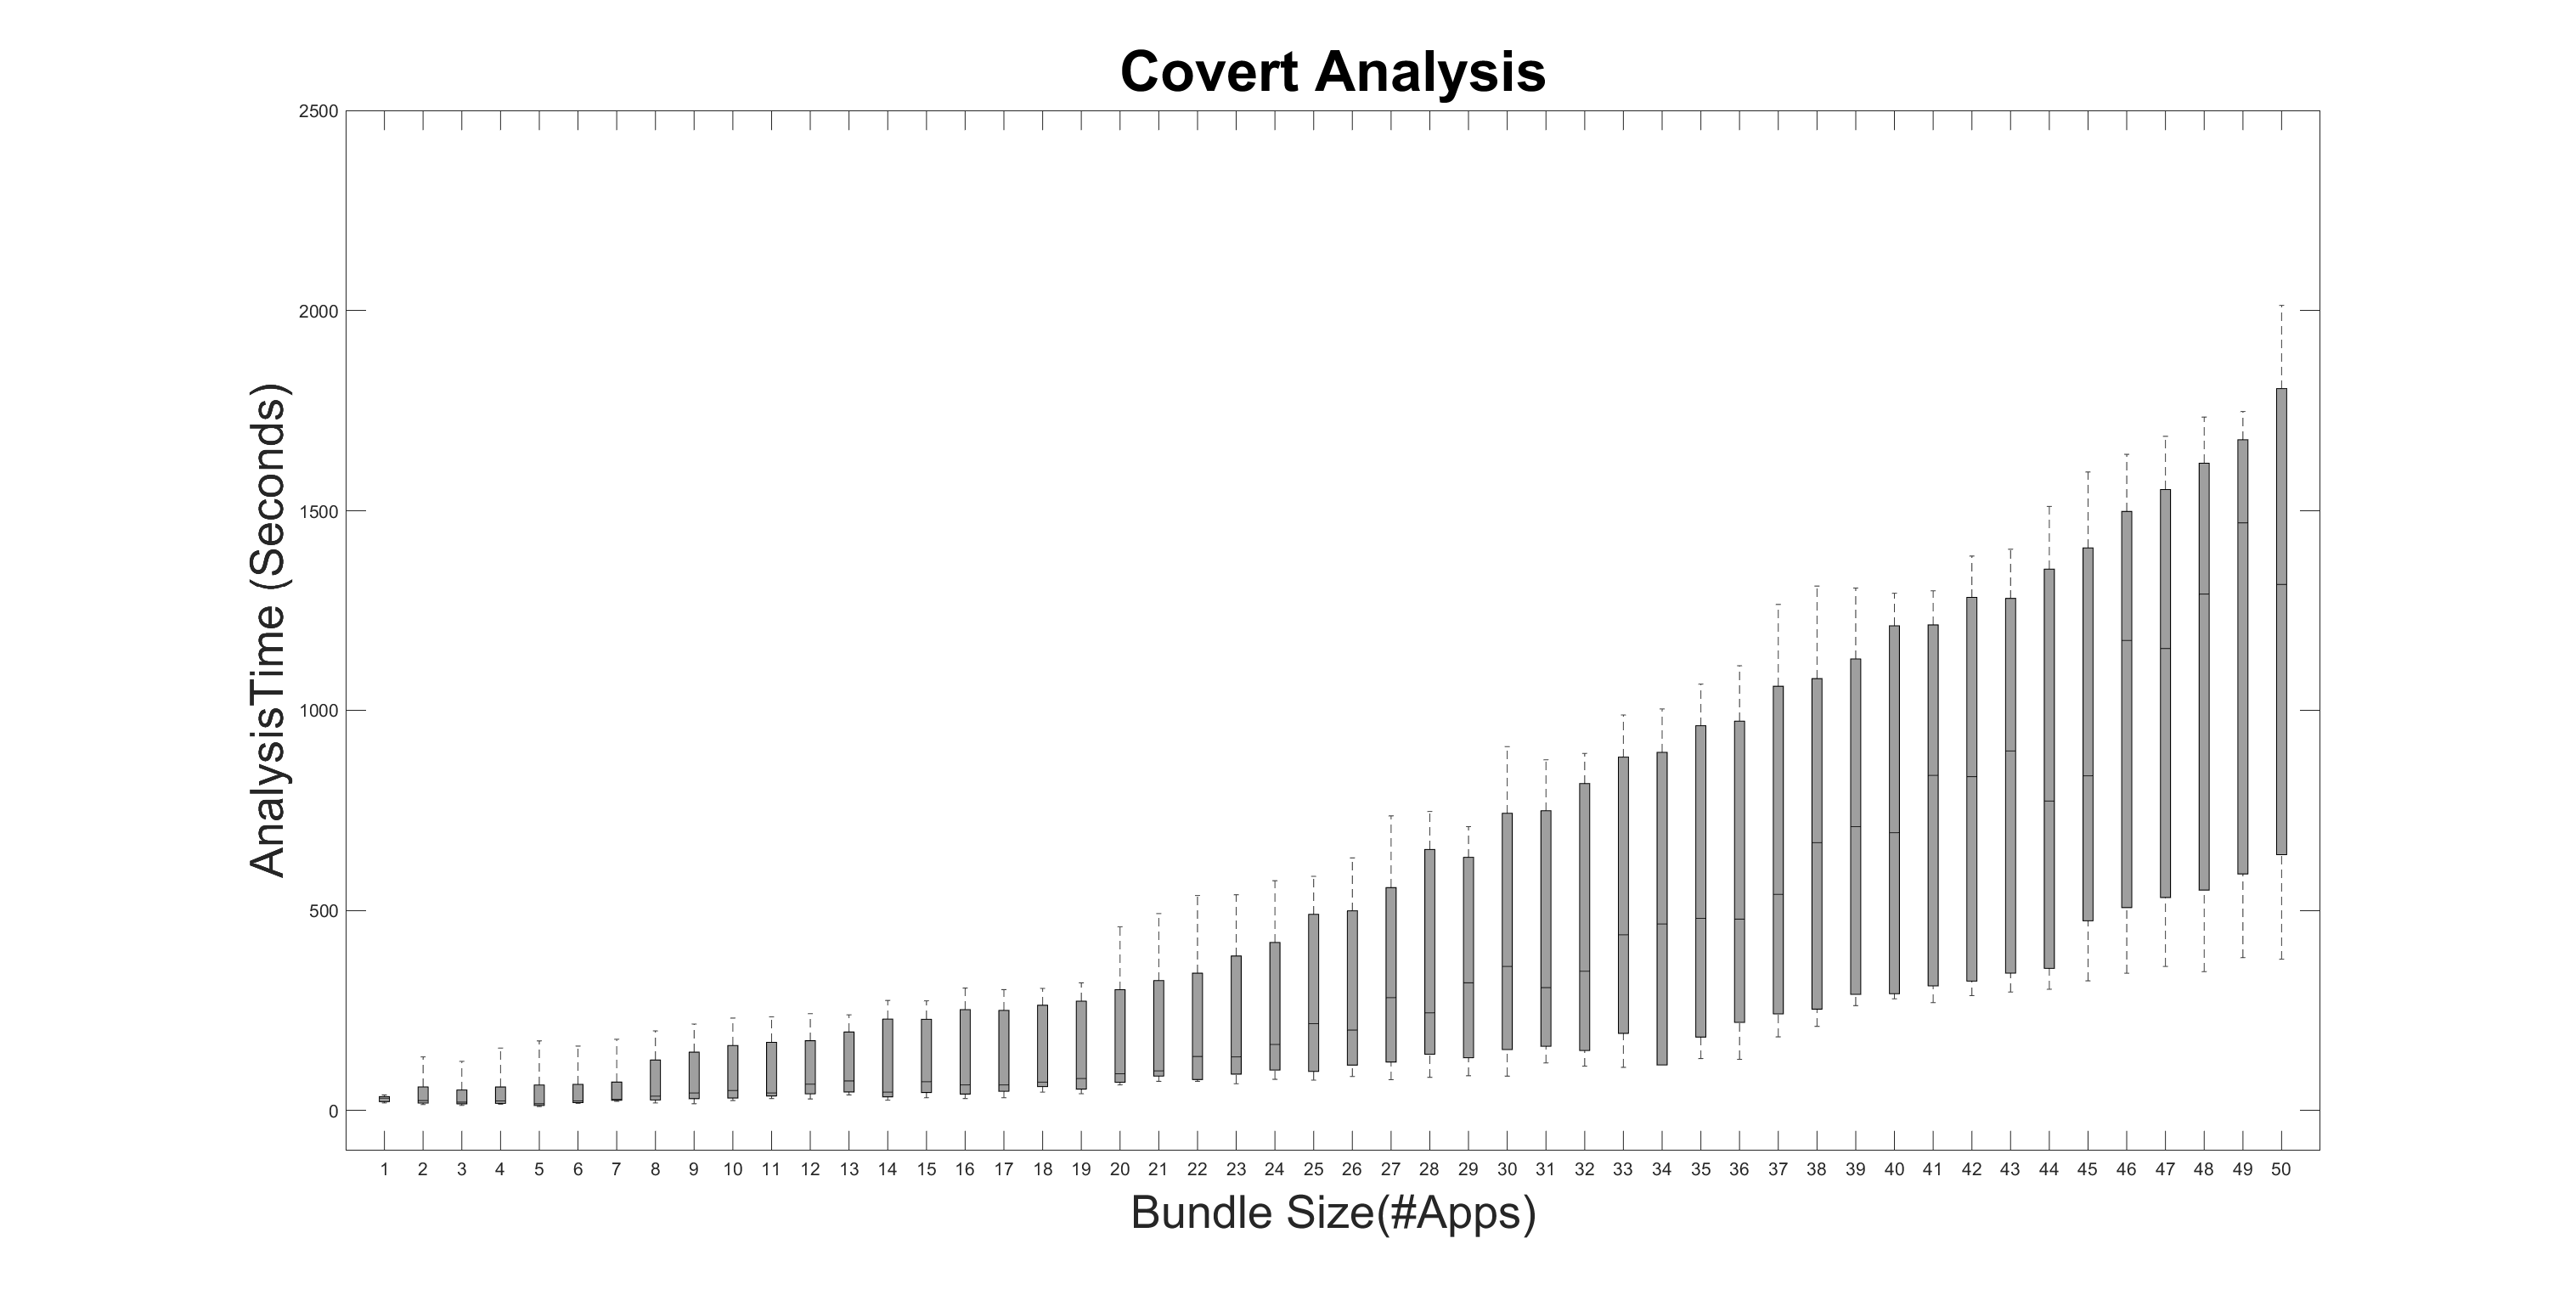
\includegraphics[width=1\linewidth]{CovertBoxPlot}
		\caption{}
	\end{subfigure}%
	\begin{subfigure}{0.5\textwidth}
		\centering
		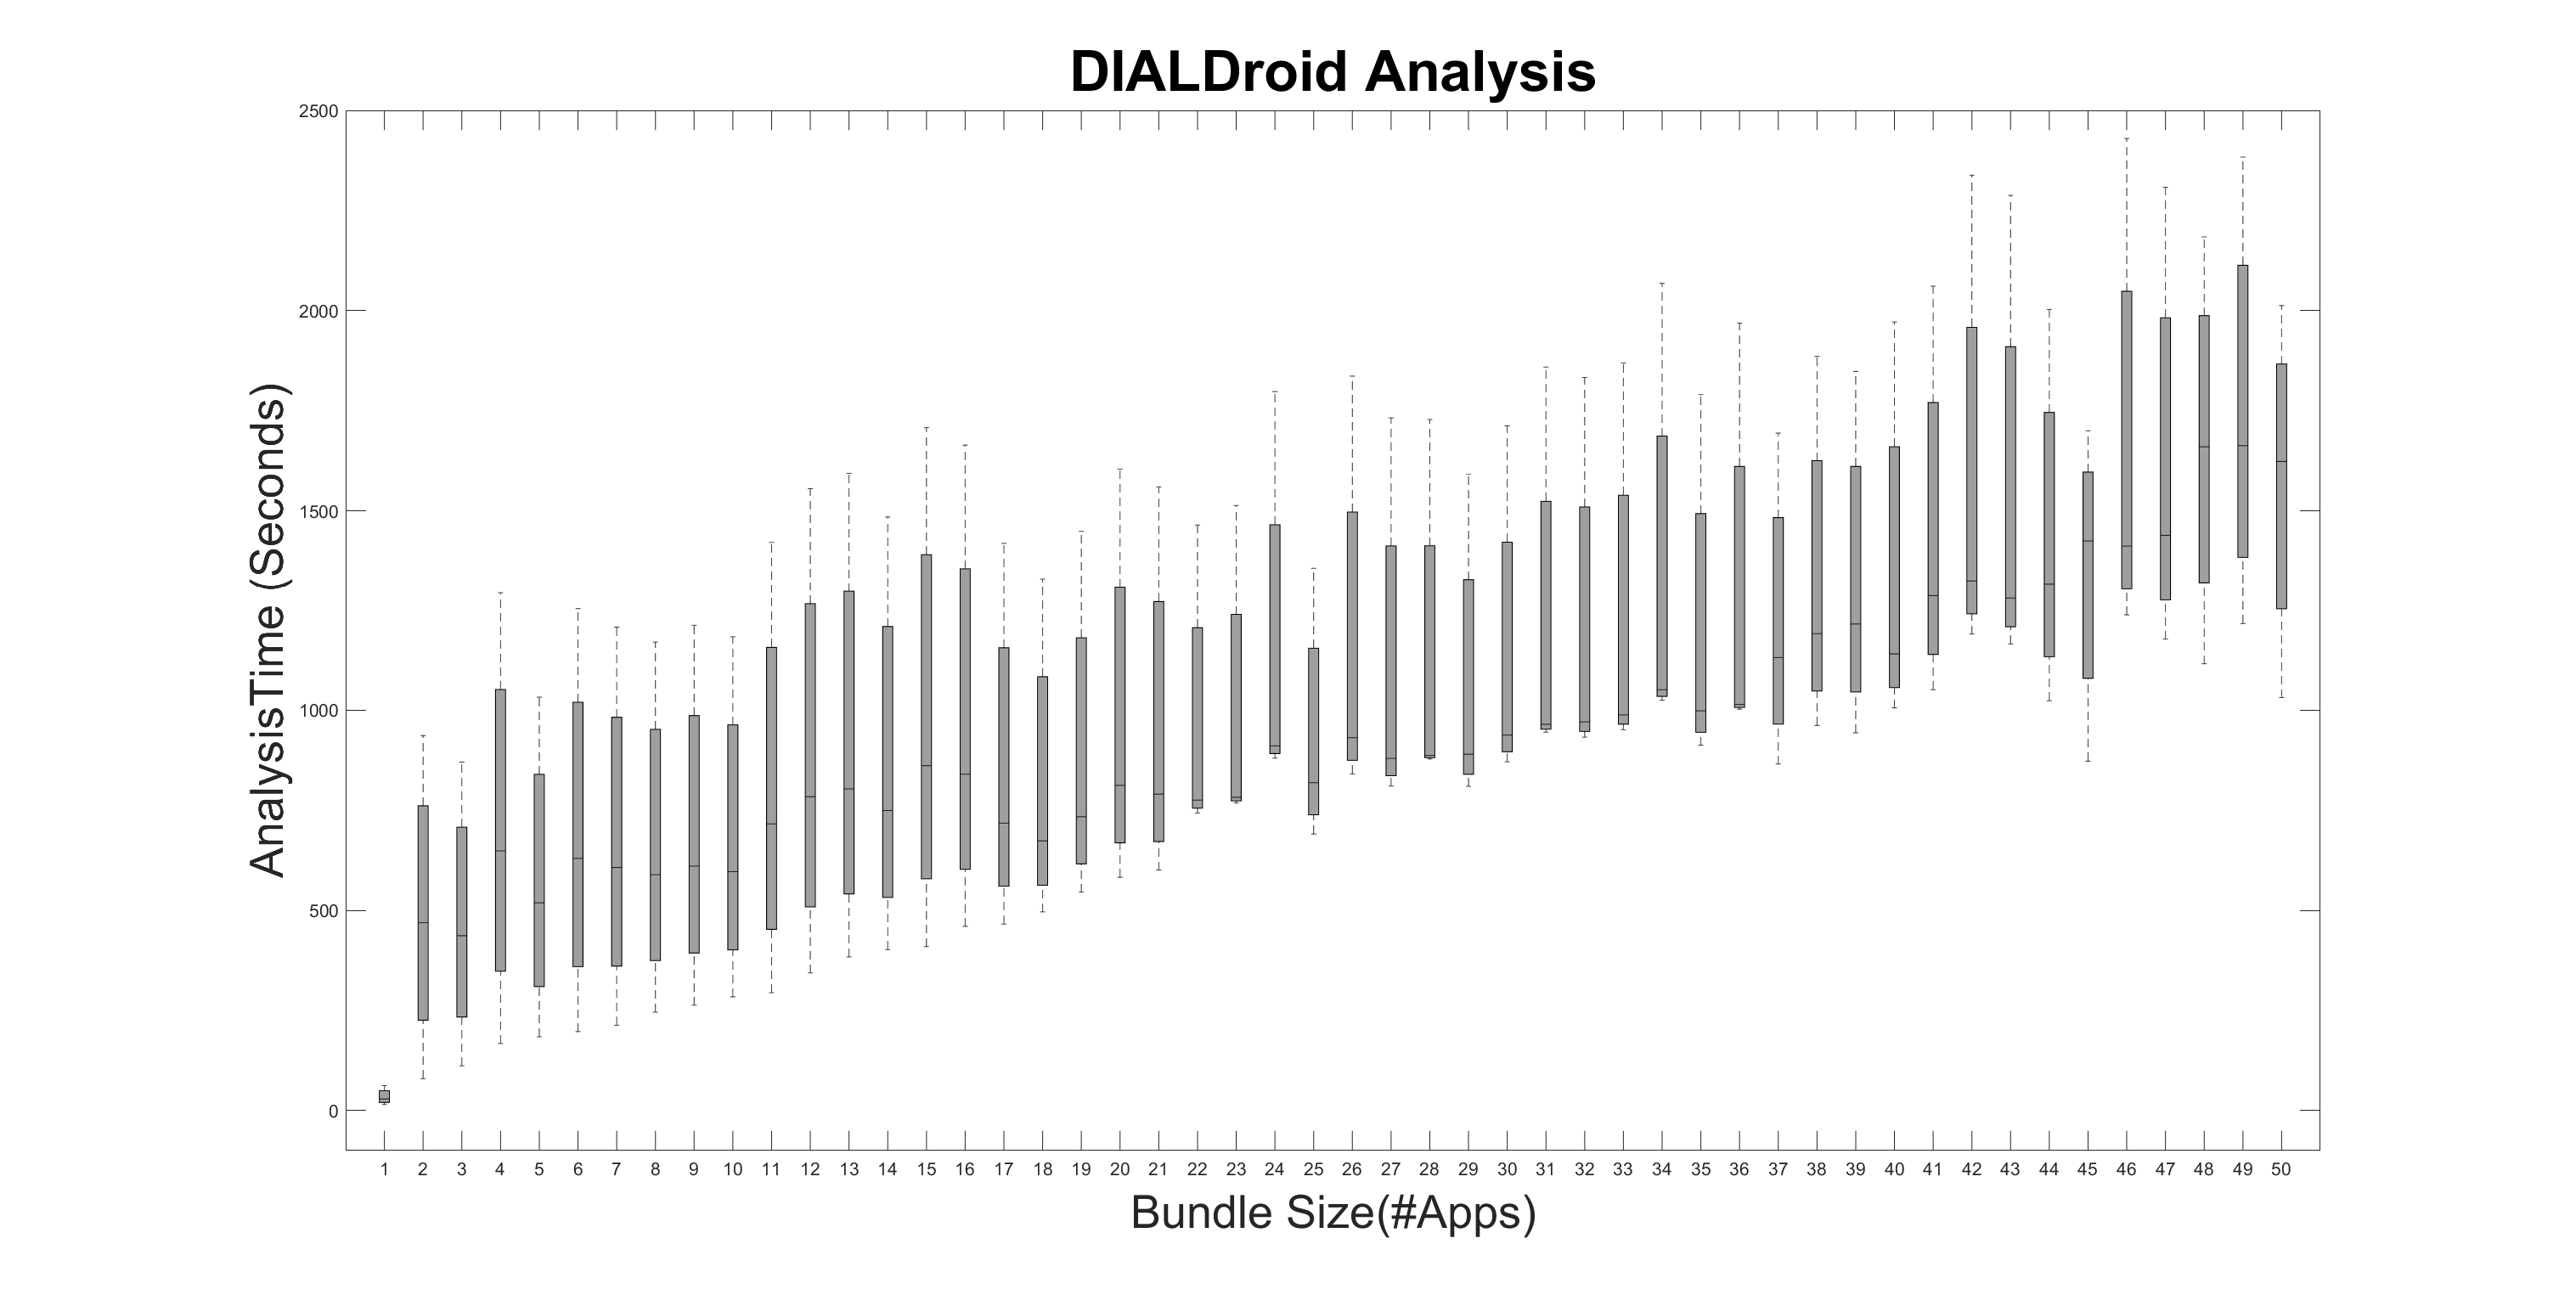
\includegraphics[width=1\linewidth]{DIALDroidBoxPlot}
		\caption{}
	\end{subfigure}
	\begin{subfigure}{0.5\textwidth}
		\centering
		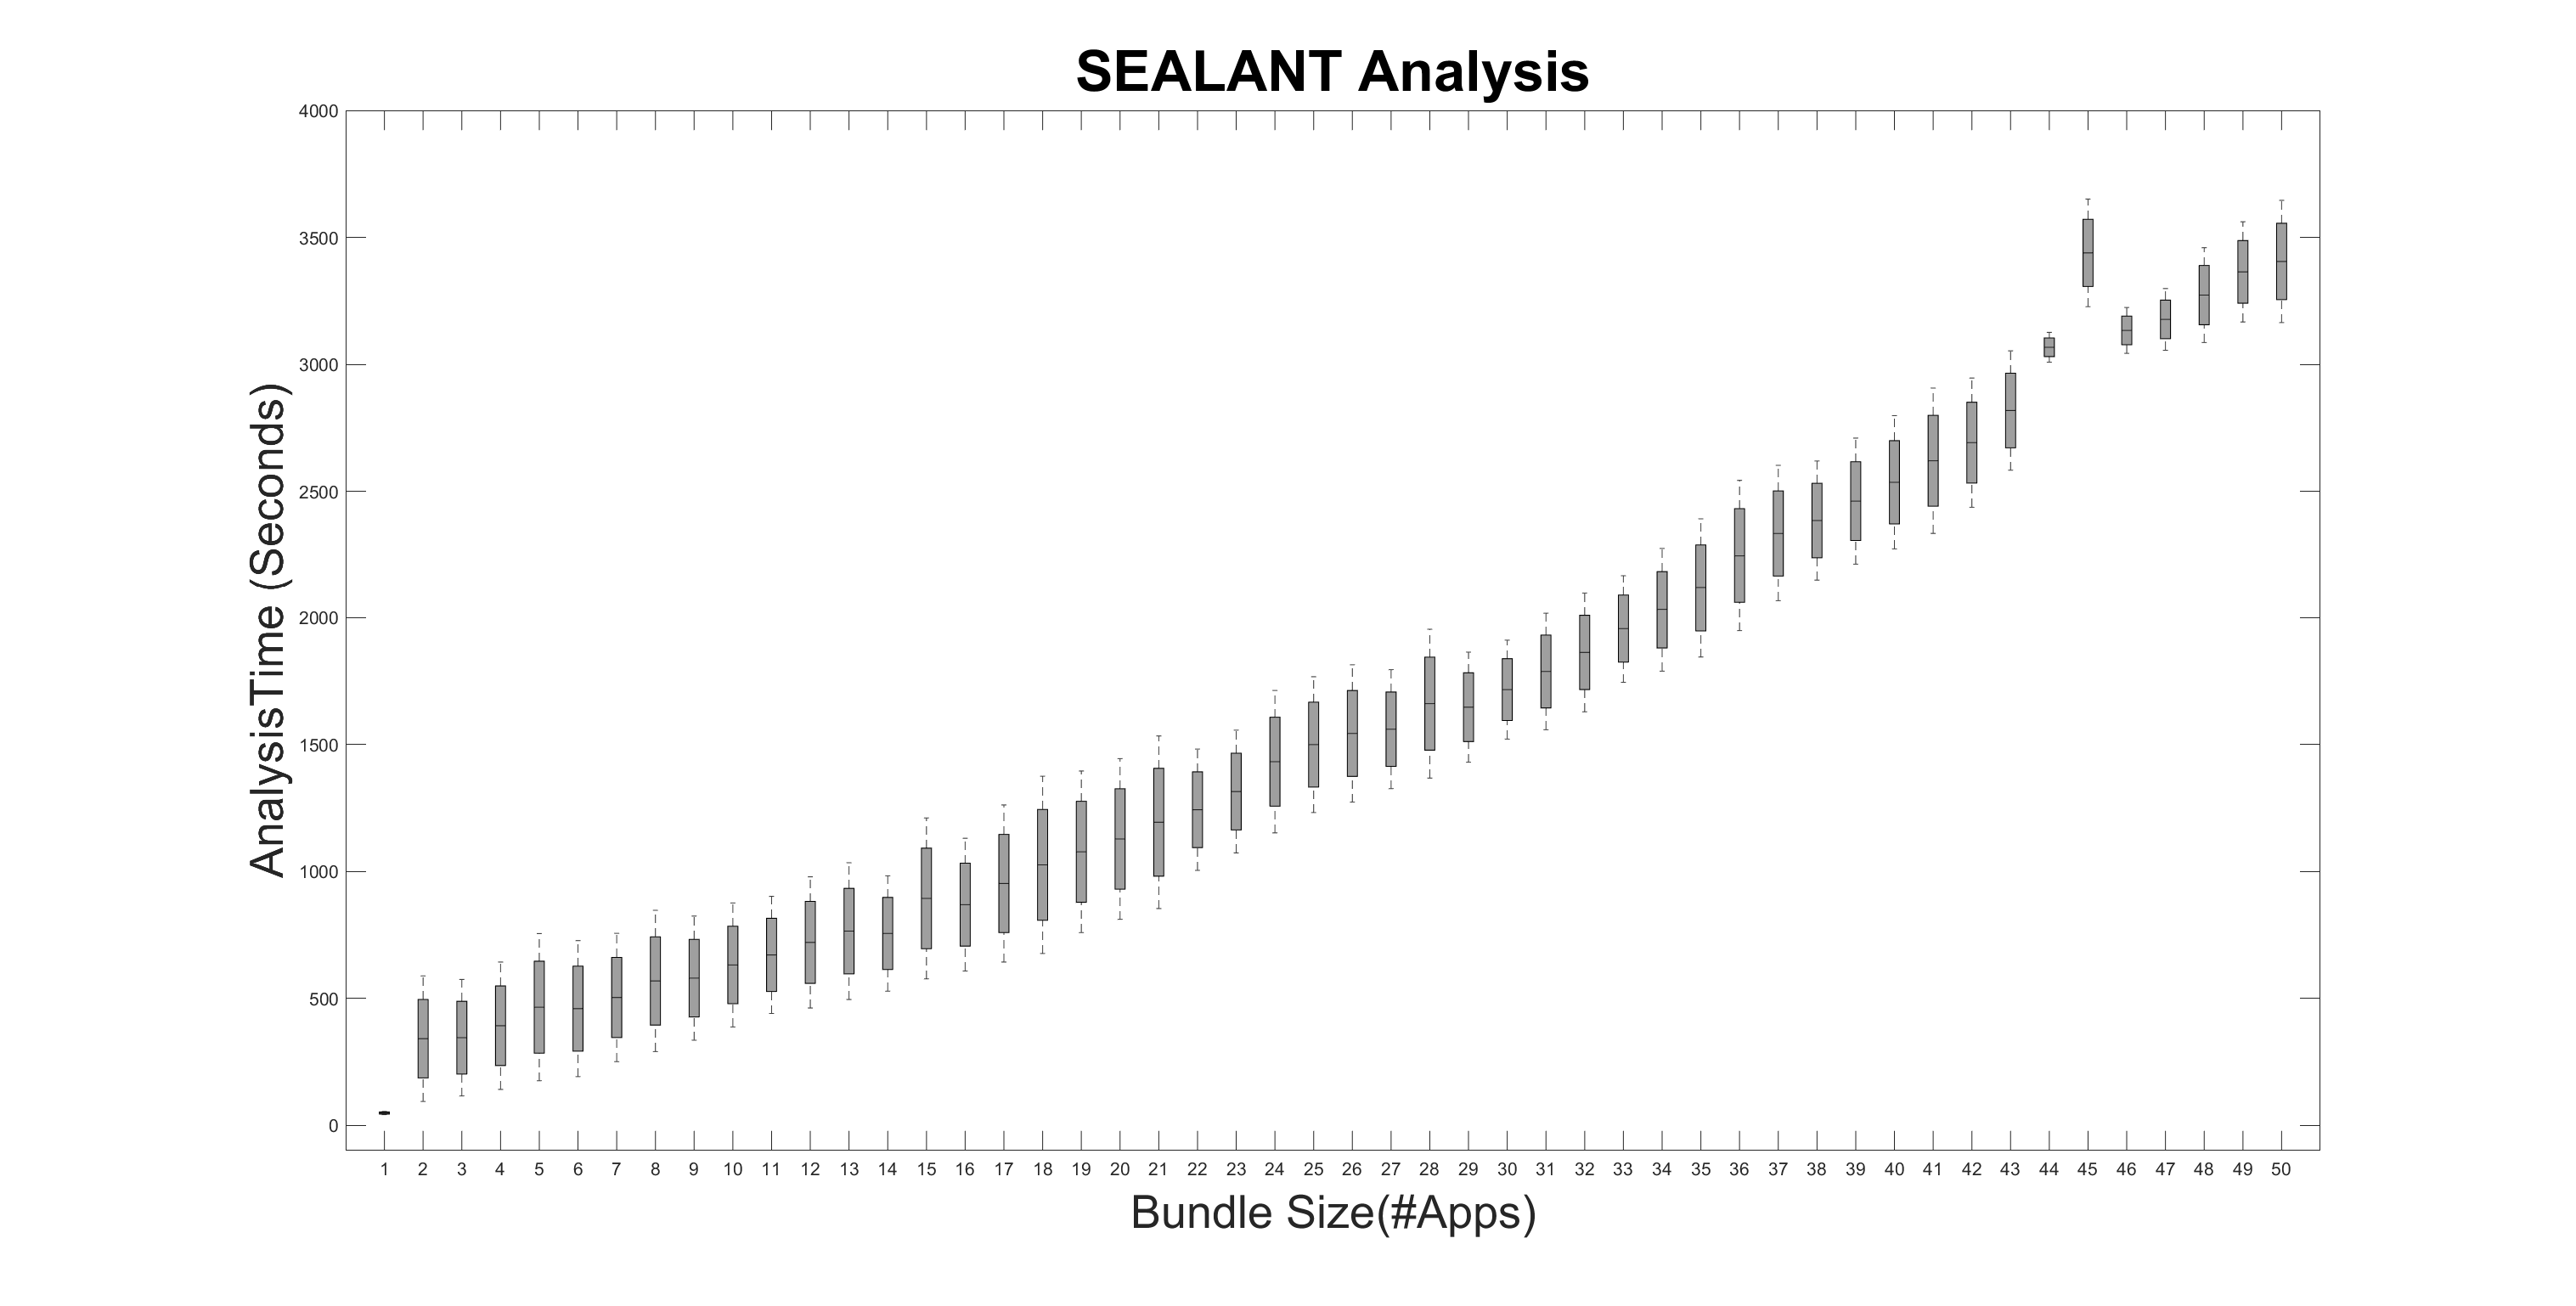
\includegraphics[width=1\linewidth]{SEALANTBoxPlot}
		\caption{}
	\end{subfigure}%
	\begin{subfigure}{0.5\textwidth}
		\centering
		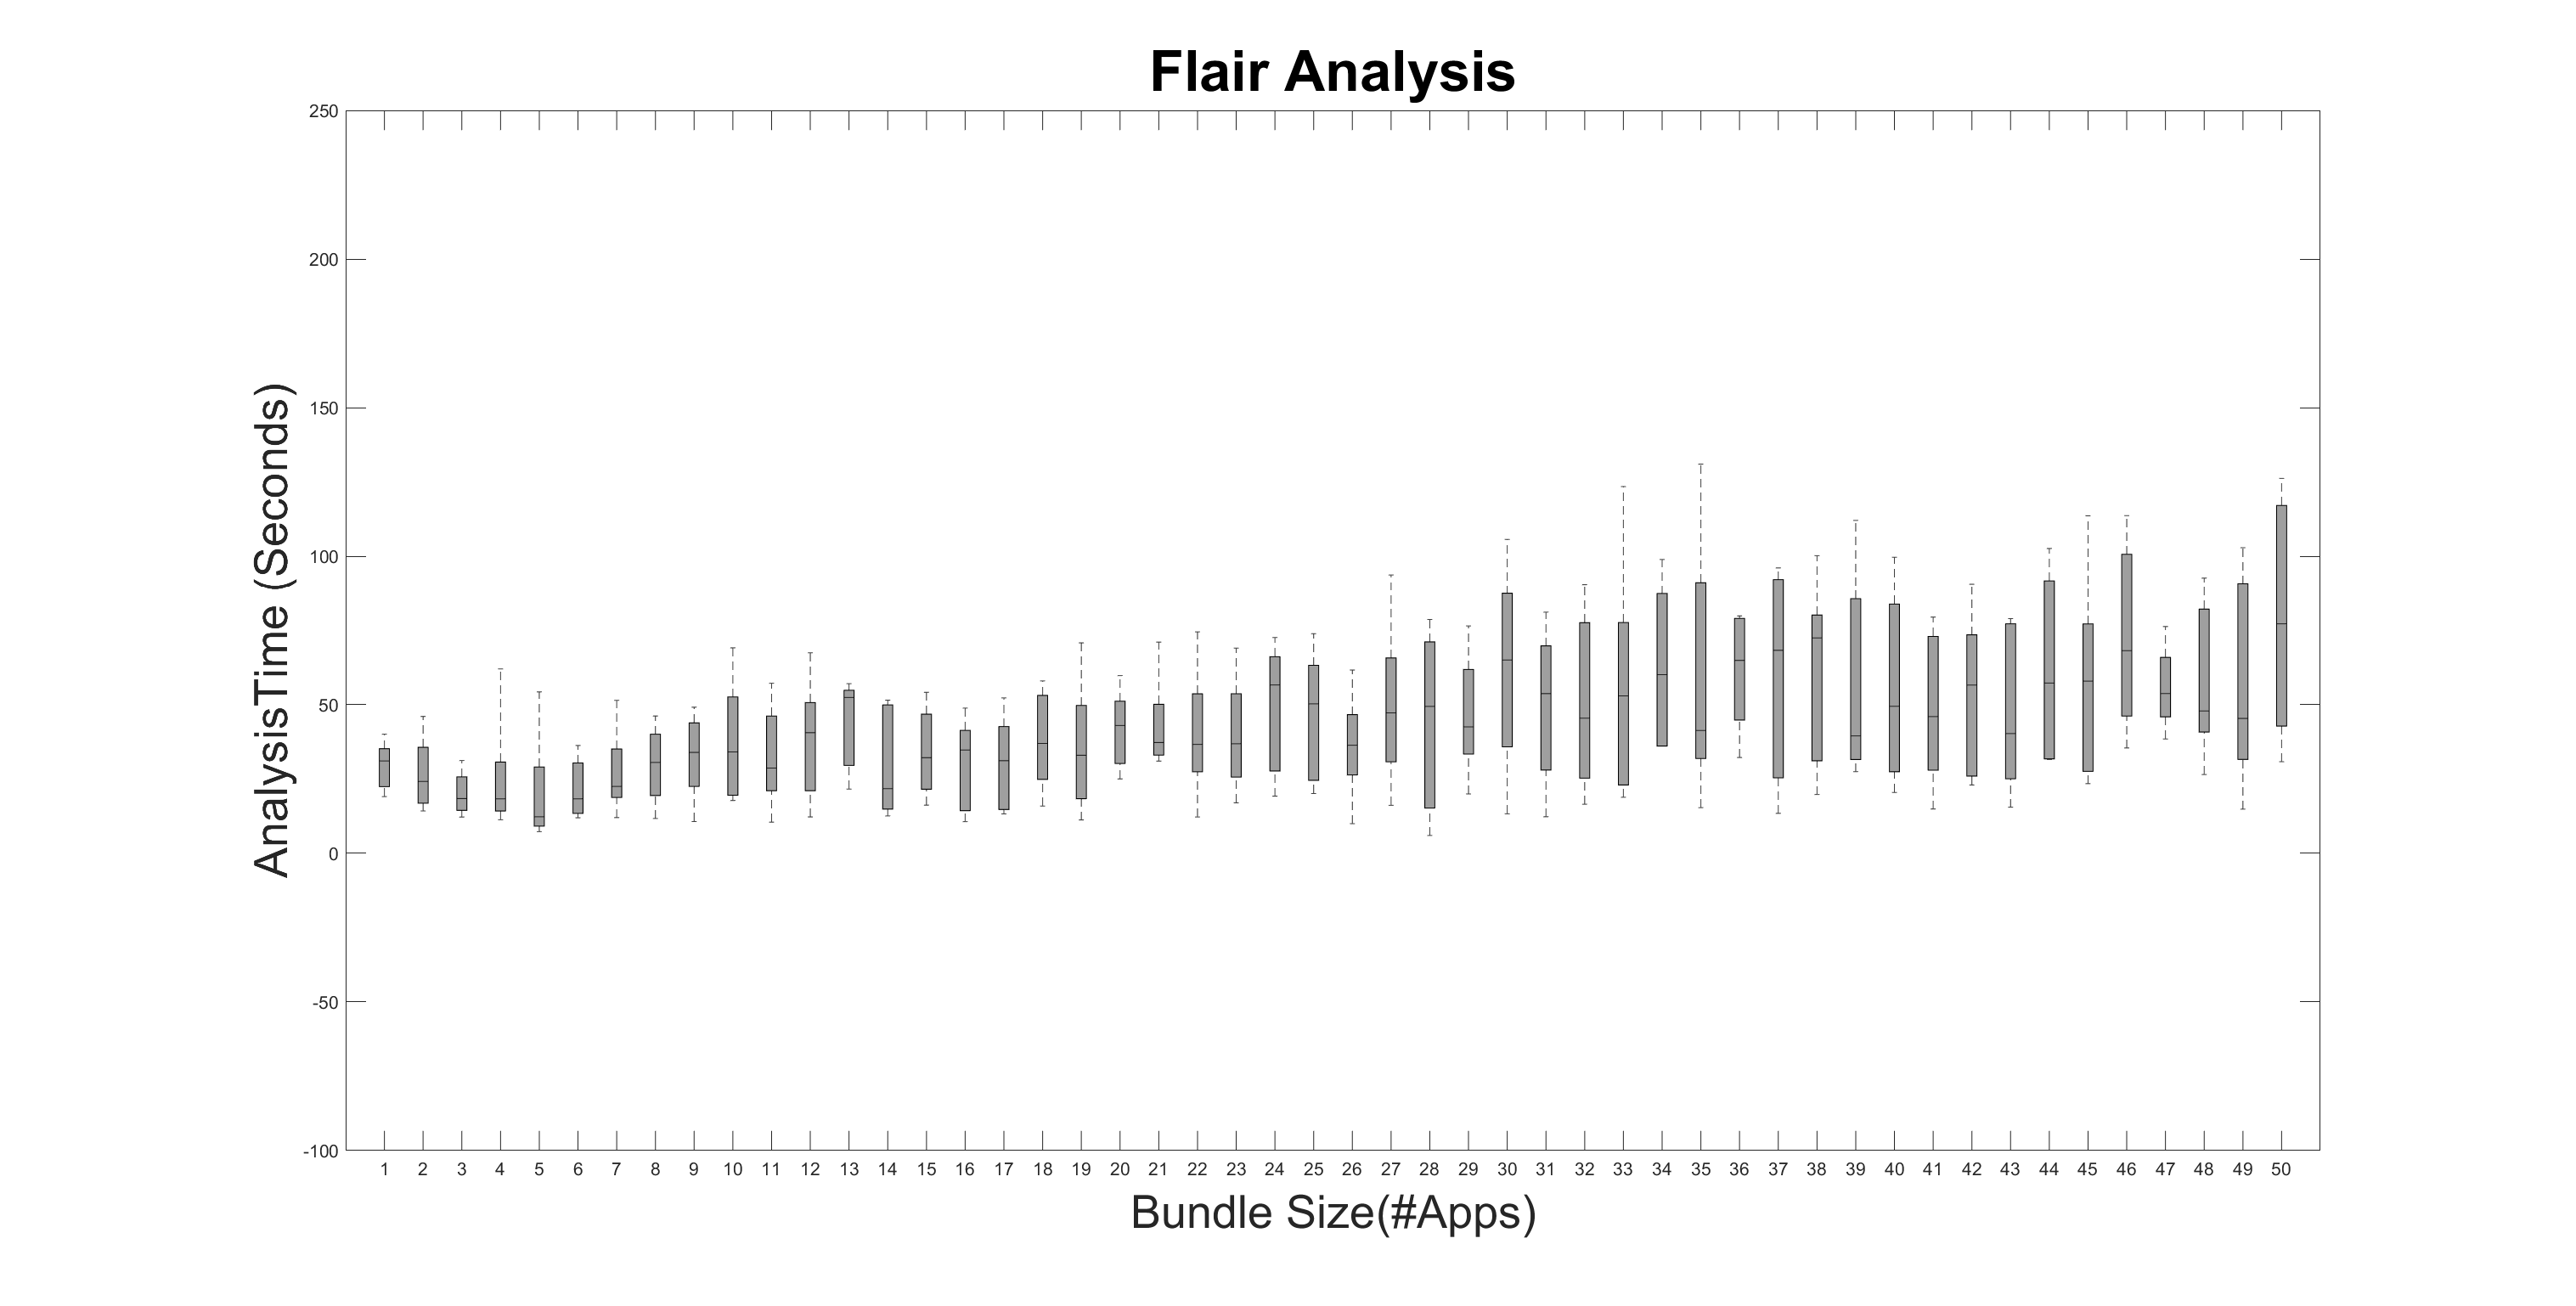
\includegraphics[width=1\linewidth]{FlairBoxPlot}
		\caption{}
	\end{subfigure}
	
	\label{figure:1}
	\caption{Box plot graphs showing tool analysis times for various tools.}
\end{figure}

\twocolumn
	%Average Analysis Time Graph
	\begin{figure}
		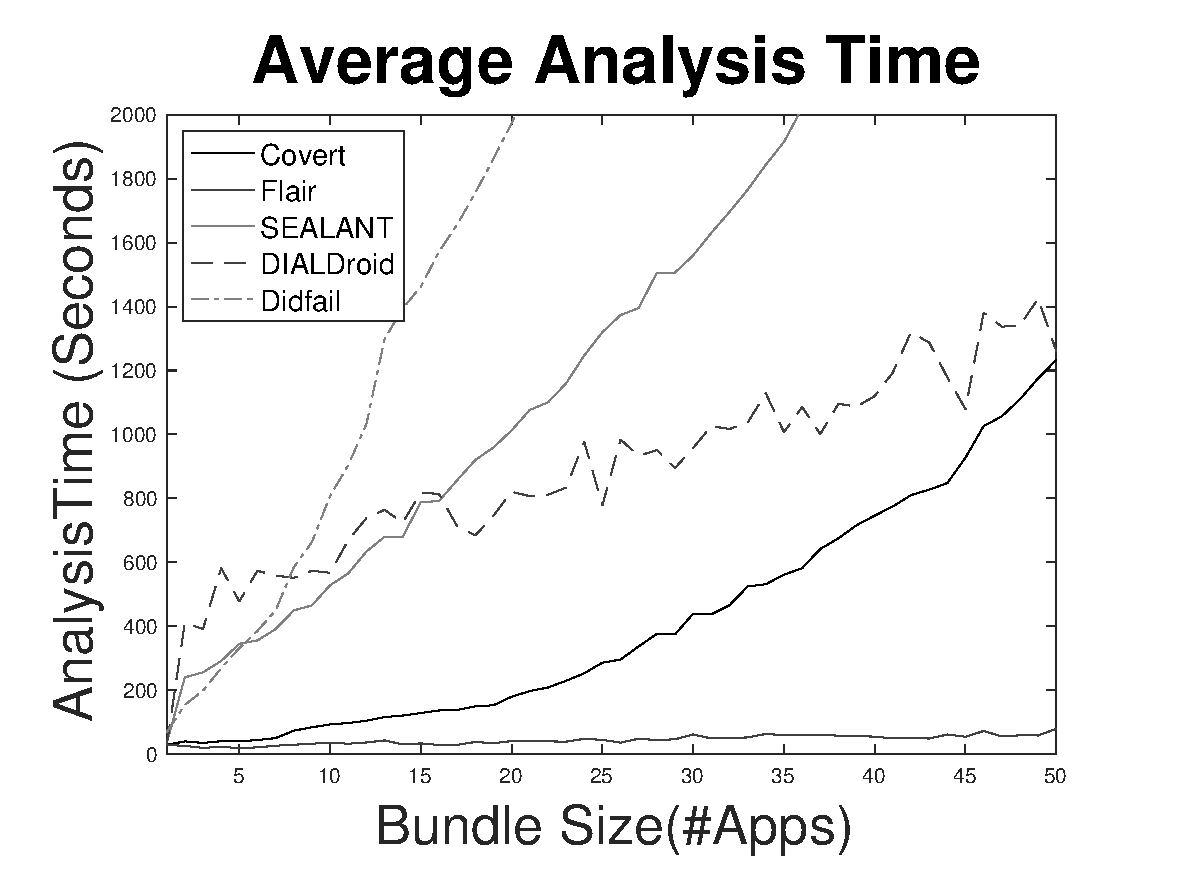
\includegraphics[width=\linewidth]{AverageGraph}
		\label{figure:2}
		\caption{Average analysis times for tools.}
	\end{figure}
	
	\subsection{Question 1:}
		We first look to evaluate the analysis time of Flair in relation to Covert, DIALDroid, and SEALANT. The box plot graphs presented in Figure 1 show the spread of analysis times for each tool. This data is presented in accordance with Figure 2 which represents the average analysis time of all tests run for all tools. These results show that Flair has a much smaller spread of analysis time across bundles, and much faster analysis times when analyzing bundles in an iterative fashion. Flair is able to analyze each application added to a bundle far faster since it only has to analyze the one application that was added, whereas the other tools analyze the entire bundle plus an additional application.\\
		It is noticed in Figure 2 that SEALANT and Covert follow similar trends, except SEALANT shows much greater analysis times. This is most likely because SEALANT is built on top of Covert and runs Covert within its Analysis tool. In addition to Covert SEALANT also runs IC3 in its analyzer tool. The trend of covert is maintained in the data, but extra time is added with the addition of the IC3. DIALDroid follows a trend which appears to cause a great increase in time during the first few applications of a bundle. After those first few applications, DIALDroid increases at a much slower rate. Didfail's analysis times grows far faster than any of the other tools. Though it is not presented in \ref{figure:2}, Didfail fails to make it all the way to fifty applications. It could only get to thirty applications before failing to analyze any bundle that was larger. Flair maintains a near horizontal trend far below the other average times.
		
	\subsection{Question 2:}
	
		%Table for the Failure Rate of Tools
		\begin{table}[h]
		\begin{center}
			\begin{tabular}{ |c c| }
				\hline
				Tool & Percentage Failed\\
				\hline
				Covert & 0\\
				DIALDroid & 32.19\\
				SEALANT & 0\\
				Didfail & 0\\
				Flair & 0\\
				\hline
			\end{tabular}		
			\end{center}
			\label{table:2}
			\caption{Rate of Failure for tools.}
		\end{table}
		
		To assess the rate of failure in the various tools we used the methods described in \ref{methods} to find the percentage of applications in each test which failed. The data which was collected is presented in \ref{table:2}. This data shows that while Covert, SEALANT, Didfail, and Flair do not fail to analyze any of the applications, DIALDroid failed a significant \textit{32.19 percent\textbf{(NOT FINAL NUMBER)}} of applications on average across all runs. This was primarily because DIALDroid would attempt to allocate more than our allotted 14 GB of memory, which was more than twice that allocated to any of the other tools. SEALANT, Covert, Didfail, and Flair all were able to run without any memory issues with far less memory. Therefore, Flair is able to analyze applications as reliably in terms of failure rate as well as SEALANT, Covert, and Didfail, while analyzing applications more reliably than DIALDroid.
		
	\subsection{Question 3:}
		text
	\subsection{Question 4:}
		text


\section[3]{Conclusion}
Here we will have a conclusion.


\end{document}

